% Appendix A

\chapter{Dictionary Learning Level Set} % Main appendix title

\label{AppendixDL2S} % For referencing this appendix elsewhere, use \ref{AppendixA}

\lhead{Appendix A. \emph{DL2S}} % This is for the header on each page - perhaps a shortened title

\section{Dictionary Learning Level Sets (DL2S)}

The primary motivation for DL2S is similar to that of L2S-- performing segmentation in presence of intensity inhomogeneity. In L2S\cite{mukherjee_L2S}, we generalized the Chan-Vese model by approximating the foreground and background regions as a piecewise polynomial function  computed via linear combination of a few Legendre basis functions. This can be viewed from the perspective of low dimensional approximation of a signal.  While Chan-Vese's method is a form of extreme dimensionality reduction (due to the piecewise constant assumption), L2S achieves a balance between reduction of dimensionality and accurate intensity modeling. 

Despite its merits, L2S suffers from certain issues. First, the segmentation quality relies heavily on the number of chosen basis functions. Second,  L2S suffers from scalability issues since the pre-specified bases cannot represent any arbitrary intensity variation. As it turns out, recent research in the field of sparse modeling and dictionary learning\cite{sparse_face,dl_algo,elad_denoising,dl_restoration,elad_ksvd} have shown that for a given set of training data, one can obtain an optimal set of basis elements (atoms) to represent a signal. This is the main highlight of DL2S --\emph{instead of explicitly specifying the set of basis elements, we estimate an optimal set of bases from the set of training images using dictionary learning}.
\begin{figure}[t]
\centering
	\renewcommand{\tabcolsep}{0.05cm}
	\renewcommand{\arraystretch}{0.05}
	\begin{tabular}{@{}ccc@{}}
		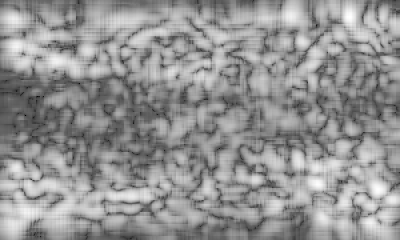
\includegraphics[width=.3\linewidth]{./images/DL2S/compare/vessINVIVO2_orig} &
		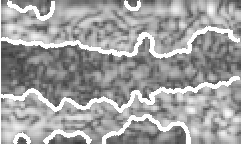
\includegraphics[width=.3\linewidth]{./images/DL2S/compare/vessINVIVO2_CV} &
		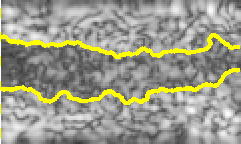
\includegraphics[width=.3\linewidth]{./images/DL2S/compare/vessINVIVO2_DL} 
		\\
		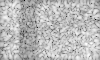
\includegraphics[width=.3\linewidth]{./images/DL2S/compare/imCyl2_orig} &		
		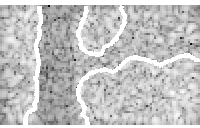
\includegraphics[width=.3\linewidth]{./images/DL2S/compare/imCyl2_CV} &
		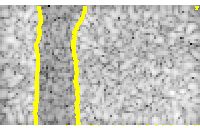
\includegraphics[width=.3\linewidth]{./images/DL2S/compare/imCyl2_DL}
		\\ 
		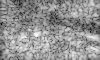
\includegraphics[width=.3\linewidth]{./images/DL2S/compare/vessFIRvol15_orig}&
 		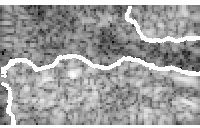
\includegraphics[width=.3\linewidth]{./images/DL2S/compare/vessFIRvol15_CV} &
		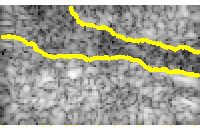
\includegraphics[width=.3\linewidth]{./images/DL2S/compare/vessFIRvol15_DL} 
	\end{tabular}
\caption[Chan-Vese vs DL2S]{Segmentation results of Chan-Vese\cite{chan_vese} (white) and DL2S (yellow) on three C-mode ultrasound images captured with a portable scanner.}
\label{fig:viz_comp}
\end{figure}
To demonstrate our technique, we choose an important segmentation problem for ultrasound imaging. Blood vessels are imaged in C-mode using a portable, low cost, battery operated ultrasound device. Our objective is to segment the vessel boundary to assist medical practitioners for performing phlebotomy application such as intravenous needle placement (see Fig.~\ref{fig:viz_comp}). Images captured using these portable devices suffer from low contrast, noise and speckle in addition to non-linear illumination of the objects which makes segmentation challenging. 
\subsection{Methodology}
A generalized version of Chan-Vese's model can be  formulated as follows:
\bea
\mathcal{E}(\phi,A,B)&=\displaystyle
\int_{\Omega}|f(\textbf{x})-\sum_{i=0}^{k}a_id_i(\textbf{x})|^2 m_1(\textbf{x}) d\textbf{x}   +\int_{\Omega}|f(\textbf{x})-\sum_{i=0}^{k}b_id_i(\textbf{x})|^2 m_2(\textbf{x}) d\textbf{x}  \nn \\
						  &+ \displaystyle \nu \int_{\Omega} |\nabla\heav(\phi)|
						   d\textbf{x} + \lambda \left(||A||_2^2+||B||_2^2\right)
\label{eq:dl_ls_mat}
\eea
Here $\mathbb{D}_k(\textbf{x})=\left[d_1(\textbf{x}),\ldots,d_k(\textbf{x})\right]^T$ is a dictionary which will be discussed in detail shortly. $d_0(\textbf{x})=\textbf{1}$. $d_1,\ldots,d_k$ are dictionary elements or atoms which are used to model the non-linearity in the intra-region intensities of the images. The third term in (\ref{eq:dl_ls_mat}) introduces smoothness in the solution, which is controlled using the parameter $\nu$. $\textbf{a}=\left[a_0,\ldots,a_k\right]^T,\textbf{b}=\left[b_0,\ldots,b_k\right]^T$ are $(k+1)$ dimension real valued coefficient vectors. The parameter $\lambda$ reduces over-fitting, by constraining the $\ell_2$ norm of the coefficient vectors.

With $k=0$, (\ref{eq:dl_ls_mat}) reduces to the piecewise constant model in (\ref{eq:chan_vese}). In other words, (\ref{eq:dl_ls_mat}) generalizes the traditional Chan-Vese technique by introducing capability to handle heterogeneous image regions. Here $d_1,\ldots,d_k$ can be interpreted as \textit{detail functions} to model the intensity variation in conjunction to the constant illumination term $d_0$. As earlier, (\ref{eq:dl_ls_mat}) can be optimized with respect to $\phi,A\; \text{and}\; B$ using alternating minimization.  

Naturally, a question arises-- how to select  $d_1(\textbf{x}),\ldots,d_k(\textbf{x})$? It was shown in \cite{mukherjee_L2S} that high quality segmentation results can be obtained by using a few Legendre basis functions. However, we hypothesize that if a dataset of example images is available, we can enhance the segmentation performance by learning an optimal set of basis functions (dictionary elements) for region intensity approximation instead of using a predefined set of basis.
For the application described in this paper, we are concerned with sets of ultrasound images, imaged using similar type of devices. The multi-depth images are captured at the same scale, and are preregistered. As a result, we have the provision to learn these functions $d_i(\textbf{x})$ directly from the dataset, rather than relying on \textit{ad hoc} procedures for selecting the same.

\subsection{Intensity modeling with dictionary learning}
Sparse coding techniques have gained popularity recently. Such algorithms have been used for a multitude of applications ranging from image denoising, inpainting, restoration, classification, retrieval etc \cite{elad_denoising,dl_algo,sparse_face,dl_restoration}. Given a set of training data, the goal of dictionary learning is to compute a set of basis elements, also called  \textit{atoms}, such that each training data can be represented as a linear combination of only a few of these atoms. The key idea is to utilize the underlying sparsity of the training data, while minimizing the reconstruction error. 
Mathematically, if $\mathbb{F}=\left[\textbf{f}_1,\ldots,\textbf{f}_N\right]$ denotes the set of $N$ discretized, vectorized and mean subtracted training images, we can use dictionary learning technique to compute the dictionary $\mathbb{D}_k=\left[\textbf{d}_1,\ldots,\textbf{d}_k\right]^T$ mentioned in (\ref{eq:dl_ls_mat}) by solving the following optimization problem
\bea
\mathbb{D}_k=\text{arg}\min_{\mathbb{D},\textbf{y}_i} \sum_{i=1}^{N}||\textbf{f}_i-\mathbb{D}^T\textbf{y}_i||_2^2 \nn \\
 \text{such that}\; ||\textbf{y}_i||_0 \leq \theta, \;\;\; \forall i=1,...,N.
 \label{eq:DL}
\eea
where $y_i$ is a coefficient vector corresponding to the $i^{th}$ training image and $\theta$ is a scalar which dictates the level of sparsity. There are a number of methods in the literature that use some approximation to solve the hard optimization problem (\ref{eq:DL}). For example, k-SVD \cite{elad_ksvd} combines a greedy methodology using orthogonal matching pursuit algorithm to provide a fast solution to this problem. Dictionary learning exploits sparsity in the data (\ref{eq:DL}) by constraining $\ell_0$ norm of the coefficients.

\subsection{DL2S curve evolution}
Let us denote $\mathbb{\hat{D}}_k=[d_0(\textbf{x})^T\; \mathbb{D}_k(\textbf{x})]^T$. We first try to minimize (\ref{eq:dl_ls_mat}) with respect to $A$ and $B$, by taking derivatives and setting the result to zero. A closed form solution  is obtained as follows:
\bea
\hat{\textbf{a}} =& \left[K+ \lambda \mathbb{I}\right]^{-1}\displaystyle\int_{\Omega} \mathbb{\hat{D}}(\textbf{x})f(\textbf{x})m_1(\textbf{x})d\textbf{x}  \\
\hat{\textbf{b}} =& \left[L+ \lambda \mathbb{I}\right]^{-1}\displaystyle\int_{\Omega}  \mathbb{\hat{D}}(\textbf{x})f(\textbf{x})m_2(\textbf{x})d\textbf{x}
\label{eq:coef_sol}
\eea
where $\left[. \right]$ denotes a matrix. $\left[K \right]$ and $\left[L \right]$ are $k\times k$ Gramian matrices \cite{gramian}, in which $(i,j)^{th}$ entries are obtained as
\bea
\left[K\right]_{i,j}= m_1(\textbf{x})\left<d_i,d_j\right> \, \text{and} \,
\left[L\right]_{i,j}= m_2(\textbf{x})\left<d_i,d_j\right>
\eea
$0\leq i,j \leq k$ and $\left<,\right>$ denotes the Euclidean inner product operator. With the updated coefficient vectors, we can now minimize (\ref{eq:dl_ls_mat}) with respect to $\phi$ using variational calculus. We obtain the following partial differential equation using gradient descent technique for minimization.
\bea
\frac{\partial \phi}{\partial t}=\left[-|f(\textbf{x})-\hat{\textbf{a}}^T\mathbb{\hat{D}}_k(\textbf{x})|^2 
						   +|f(\textbf{x})-\hat{\textbf{b}}^T\mathbb{\hat{D}}_k(\textbf{x})|^2 \right]\dirac(\phi) 
						  +  \nu \dirac(\phi)\nabla \cdot\left(\frac{\nabla\phi}{|\nabla\phi|}\right) \nn \\
\label{eq:Dl2S_final_PDE}						  
\eea
We initialize $\phi|_{t=0}=\phi_0$ and $\dfrac{\dirac(\phi)}{|\nabla \phi|}\dfrac{\partial\phi}{\partial \hat{n}}=0$ at the domain boundary. The gradient flow of DL2S is computed iteratively by discretizing (\ref{eq:Dl2S_final_PDE}) using a finite difference scheme.
\begin{figure}[t]
\centering
	\renewcommand{\tabcolsep}{0.05cm}
	\begin{tabular}{@{}cccc@{}}
		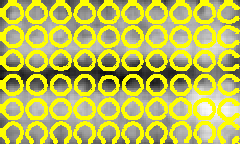
\includegraphics[width=.24\linewidth]{./images/DL2S/evolution/cylDPSS_DLevol570} &
		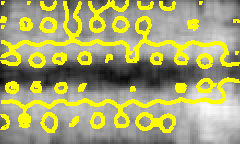
\includegraphics[width=.24\linewidth]{./images/DL2S/evolution/cylDPSS_DLevol5710} &
		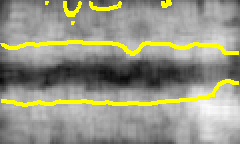
\includegraphics[width=.24\linewidth]{./images/DL2S/evolution/cylDPSS_DLevol5720} &
		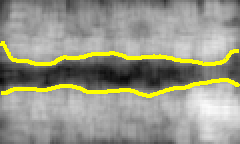
\includegraphics[width=.24\linewidth]{./images/DL2S/evolution/cylDPSS_DLevol57221} 
		\\
		\scriptsize(a) & \scriptsize (b)&\scriptsize(c)&\scriptsize(d)
	\end{tabular}
%} 
\caption[DL2S curve evolution]{Evolution steps shown for our algorithm (a) initialization, (b) iteration=20, (c) iteration=60, (d) final contour.}
\vspace{-0.5cm}
\label{fig:DL2S_curve_evol}
\end{figure}
Fig.~\ref{fig:DL2S_curve_evol} shows different steps of the curve evolution. Fig.~\ref{fig:DL2S_curve_evol}(a) shows the initialization Fig.~\ref{fig:DL2S_curve_evol}(b) and (c) shows two intermediate steps and Fig.~\ref{fig:DL2S_curve_evol}(d) shows the finally evolved curve.

\subsection{Analysis of DL2S}
\begin{figure}[th]
\centering
\renewcommand{\tabcolsep}{0.05cm}
	\begin{tabular}{@{} c@{}}
		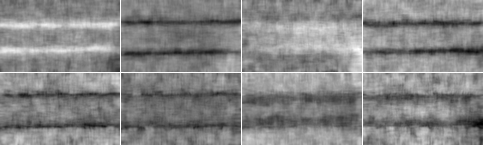
\includegraphics[width=.9\linewidth]{./images/DL2S/dataset1_dict} 
	\end{tabular}
\caption[DL2S dictionary]{Eight dictionary atoms learned from the mean subtracted images for a phantom image category.}
\label{fig:DLbasis}
\end{figure}
The Chan-Vese method performs segmentation by approximating an image $f(\textbf{x})$ by a piecewise constant image $g(\textbf{x})$. To make the model more flexible, we  add higher order terms which can capture the intensity variations in the regions. Going by the intuition of Chan and Vese, it is fair to approximate the mean image of a dataset as a piecewise constant image.  

Assuming a mean image which is approximately piecewise constant, the dictionary atoms learned from the mean subtracted dataset can be utilized to provide the non-linear variation necessary to model the intensity inhomogeneity. The energy functional in  (\ref{eq:dl_ls_mat}) essentially incorporates this idea in a mathematical framework. One can also think of the dictionary atoms as incorporating higher order details, learned to suit our dataset. The dictionary atoms computed for a particular ultrasound image dataset is shown in Fig.~\ref{fig:DLbasis}. The dictionary atoms aid in retaining the more significant image properties  and compactly represent the dataset. 

DL2S is applicable where a set of pre-registered training data is available, for example multi-depth ultrasound images of blood vessels, in temporal image sequences of biomedical objects such as carotid artery, heart videos. In applications involving a temporal image sequence, the first few frames of the can be treated as the training data to learn the dictionary, which can be exploited to segment the subsequent frames.    

\subsection{Experimental Results}
We use five different sets of images to evaluate the performance of our algorithm. Out of them, three datasets contain images of medical phantoms which mimic human veins. These phantoms are generally used by medical practitioners for device calibration. The remaining two datasets consists of human vein images, captured \textit{in vivo}. Each dataset contains approximately 18 to 60 images, captured in C-mode using a portable, battery operated ultrasound scanner. The different images in a given set correspond to the image of a vein at various depths. Note that each dataset consists of registered blood vessel images. The vessel orientation and scale are also consistent. A separate dictionary is computed using the mean subtracted images for each of the datasets. 
\begin{figure}[b]
\centering
\renewcommand{\tabcolsep}{0.05cm}
\begin{tabular}{@{}cccc@{}}
			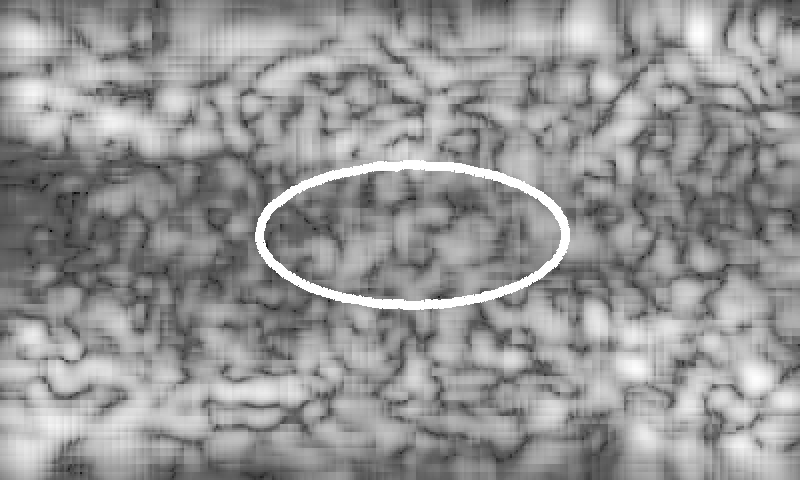
\includegraphics[width=.24\linewidth]{./images/DL2S/Initialization/init_ell} &
			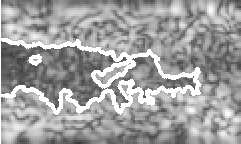
\includegraphics[width=.24\linewidth]{./images/DL2S/Initialization/vessINVIVO02_CV_ell} &
			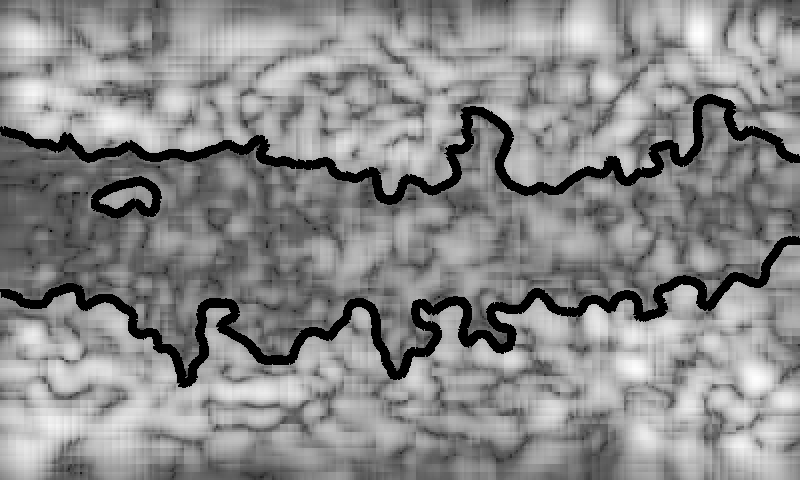
\includegraphics[width=.24\linewidth]{./images/DL2S/Initialization/vessINVIVO02_L2S_p2_ell} &
			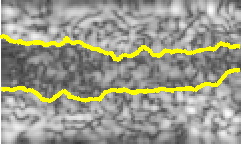
\includegraphics[width=.24\linewidth]{./images/DL2S/Initialization/vessINVIVO02_DL_ell} 
			\\ 
			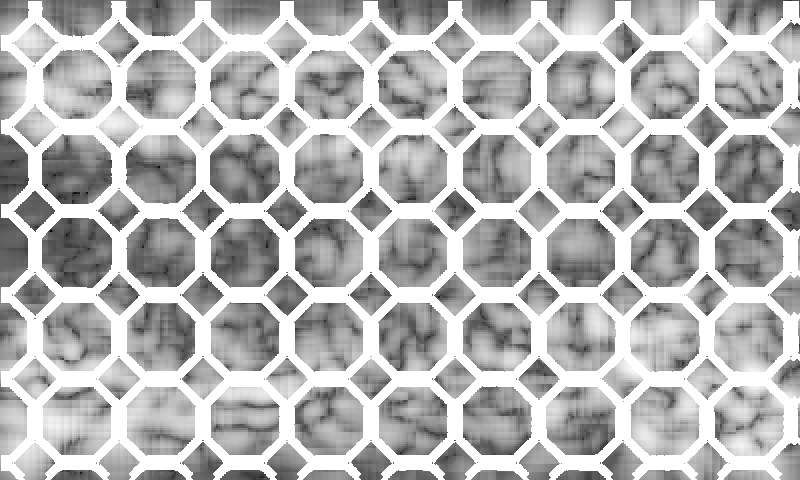
\includegraphics[width=.24\linewidth]{./images/DL2S/Initialization/init_mb} &
			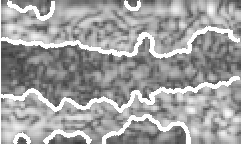
\includegraphics[width=.24\linewidth]{./images/DL2S/Initialization/vessINVIVO02_CV_mb} &
			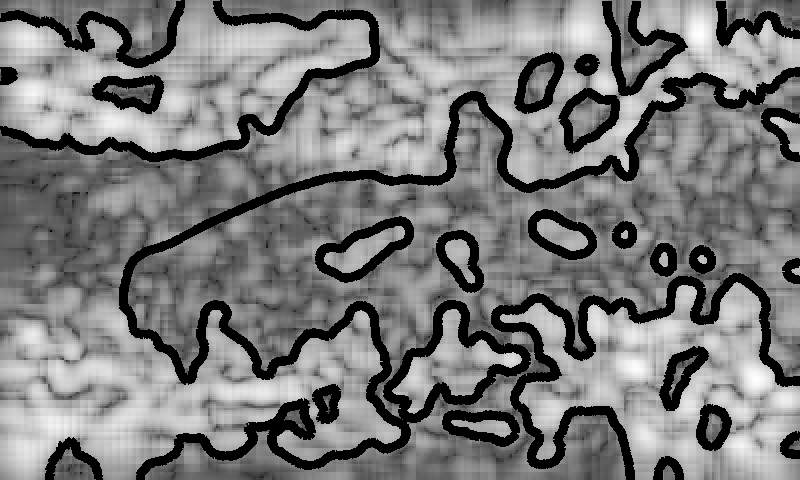
\includegraphics[width=.24\linewidth]{./images/DL2S/Initialization/vessINVIVO02_L2S_p2_mb} &
			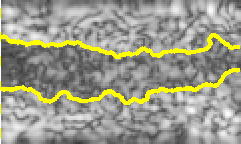
\includegraphics[width=.24\linewidth]{./images/DL2S/Initialization/vessINVIVO02_DL_mb} 
			\\
		    \scriptsize(a) & \scriptsize (b) &\scriptsize (c) & \scriptsize (d)
\end{tabular}
\caption[DL2S initialization robustness]{Comparison of segmentation results using manual and automatic initialization methods. (a) initialized contour (b) segmentation results of Chan-Vese (white), (c) segmentation via L2S (black) and (d) segmentation via DL2S model (yellow)}
\label{fig:init_compare}
\end{figure}

\textbf{Dependency on contour initialization}: We show the performance of our algorithm using both manual and automatic initialization methods. The segmentation results with manual and automatic initialization for Chan-Vese\cite{chan_vese}, L2S \cite{mukherjee_L2S} and DL2S are shown in Fig.~ \ref{fig:init_compare} for the same image. We observe that the segmentation performance of L2S drops significantly for automatic initialization, which is also true for Chan-Vese method. In comparison DL2S has similar segmentation results for both initialization technique. Quantitative evaluation of performance based on initialization is provided in Table I.
\begin{figure}[t]
\centering
	\renewcommand{\tabcolsep}{0.05cm}
	\begin{tabular}{@{}cccc@{}}
		%\raisebox{0.2in}{(a)} &
		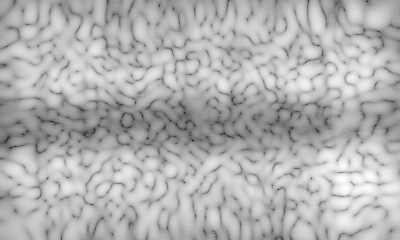
\includegraphics[width=.23\linewidth]{./images/DL2S/compare/cylNORM57_orig} &
		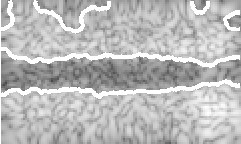
\includegraphics[width=.23\linewidth]{./images/DL2S/compare/cylNORM57_CV} &
		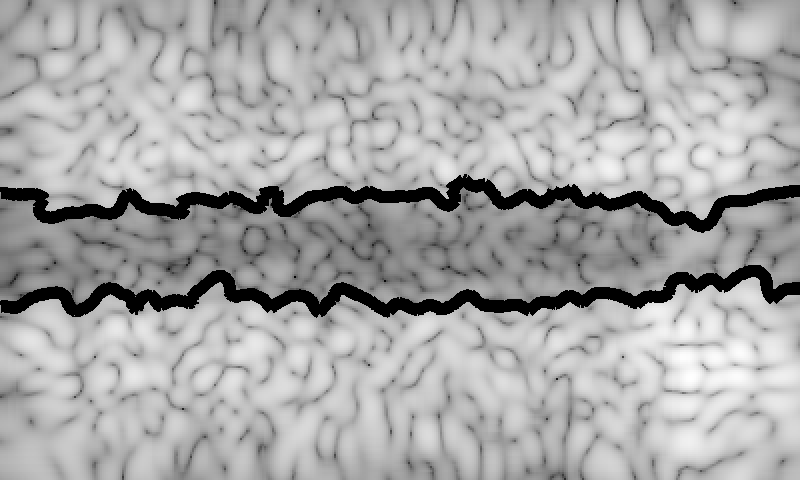
\includegraphics[width=.23\linewidth]{./images/DL2S/compare/cylNORM57_L2S_p2_c} &
		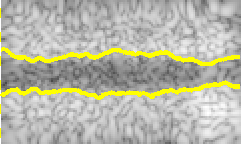
\includegraphics[width=.23\linewidth]{./images/DL2S/compare/cylNORM57_DL} 
		\\
		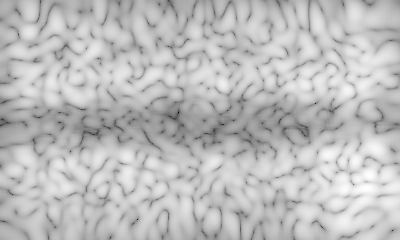
\includegraphics[width=.23\linewidth]{./images/DL2S/compare/cylNORM59_orig} &
		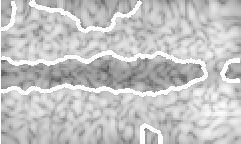
\includegraphics[width=.23\linewidth]{./images/DL2S/compare/cylNORM59_CV} &
		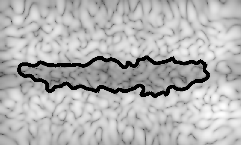
\includegraphics[width=.23\linewidth]{./images/DL2S/compare/cylNORM59_L2S_p2_c} &
		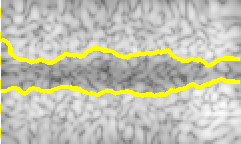
\includegraphics[width=.23\linewidth]{./images/DL2S/compare/cylNORM59_DL} 
		\\
		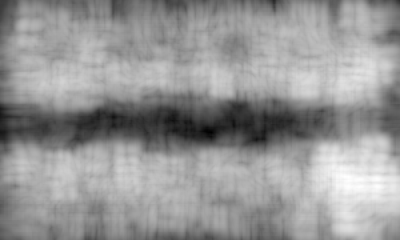
\includegraphics[width=.23\linewidth]{./images/DL2S/compare/cylDPSS58_orig} &
		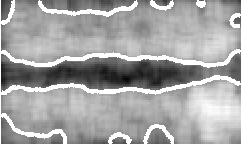
\includegraphics[width=.23\linewidth]{./images/DL2S/compare/cylDPSS58_CV} &
		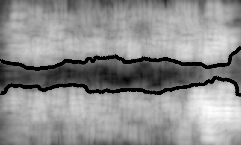
\includegraphics[width=.23\linewidth]{./images/DL2S/compare/cylDPSS58_L2S_p2_c}&				
		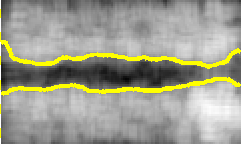
\includegraphics[width=.23\linewidth]{./images/DL2S/compare/cylDPSS58_DL}
		\\
		\includegraphics[width=.23\linewidth]{./images/DL2S/compare/vessFIRvol10_orig} &
		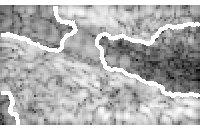
\includegraphics[width=.23\linewidth]{./images/DL2S/compare/vessFIRvol10_CV} &
		\includegraphics[width=.23\linewidth]{./images/DL2S/compare/vessFIRvol10_L2S_p2_c} &
		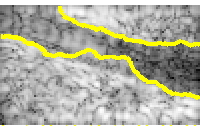
\includegraphics[width=.23\linewidth]{./images/DL2S/compare/vessFIRvol10_DL} 
		\\		
		\includegraphics[width=.23\linewidth]{./images/DL2S/compare/vessFIRvol18_orig} &
		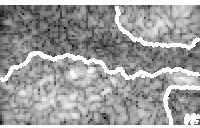
\includegraphics[width=.23\linewidth]{./images/DL2S/compare/vessFIRvol18_CV} &		
		\includegraphics[width=.23\linewidth]{./images/DL2S/compare/vessFIRvol18_L2S_p2_c} &		
		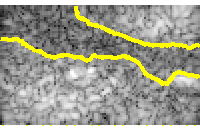
\includegraphics[width=.23\linewidth]{./images/DL2S/compare/vessFIRvol18_DL} 
		\\		
		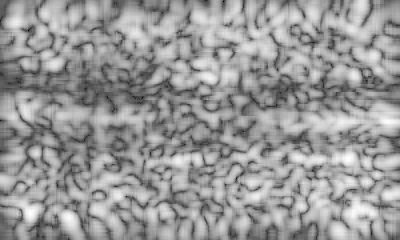
\includegraphics[width=.23\linewidth]{./images/DL2S/compare/vessINVIVO15_orig} &
		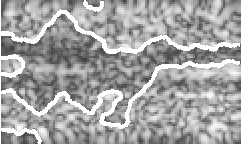
\includegraphics[width=.23\linewidth]{./images/DL2S/compare/vessINVIVO15_CV} &		
		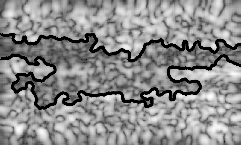
\includegraphics[width=.23\linewidth]{./images/DL2S/compare/vessINVIVO15_L2S_p2_c} &		
		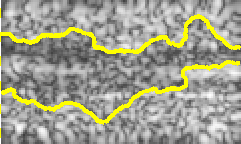
\includegraphics[width=.23\linewidth]{./images/DL2S/compare/vessINVIVO15_DL} 
		\\		
		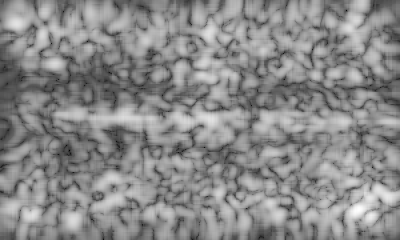
\includegraphics[width=.23\linewidth]{./images/DL2S/compare/vessINVIVO17_orig} &
		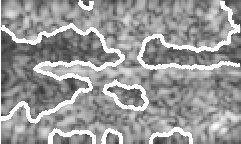
\includegraphics[width=.23\linewidth]{./images/DL2S/compare/vessINVIVO17_CV}   &
		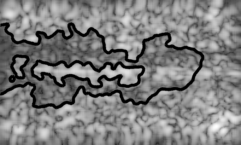
\includegraphics[width=.23\linewidth]{./images/DL2S/compare/vessINVIVO17_L2S_p2_c} & 
		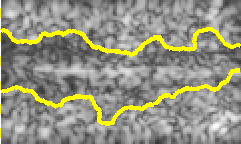
\includegraphics[width=.23\linewidth]{./images/DL2S/compare/vessINVIVO17_DL} 
	\end{tabular}
\caption[Qualitative comparison of DL2S]{Segmentation comparison of DL2S with Chan-Vese and L2S is shown here. The original C-mode ultrasound images captured with a portable scanner are shown in the first column. Segmentation results of Chan-Vese (white), L2S (black) and DL2S model (yellow) on these images are shown in columns 2, 3 and 4 respectively.}
\label{fig:seg_comp}
\end{figure}

\textbf{Dependency on dictionary size}: We perform sensitivity analysis experiment to study the performance of the segmentation algorithm  with changing dictionary size. The Dice coefficient are plotted (along Y-axis) for L2S \cite{mukherjee_L2S} (Fig.~\ref{fig:quant_compPolydeg} (a)) ans DL2S (Fig.~\ref{fig:quant_compPolydeg} (b)) to show the performance with changing basis / dictionary size (along X-axis) for 7 randomly chosen images. In comparison to L2S, where performance decreases with increasing number of basis functions, DL2S exhibits a more stable performance. Based on experiment evaluation, we fix the number of dictionary elements $k=8$ which is at most 50\% of the size of the smallest dataset. We choose sparsity inducing parameter $\theta=3$ such that about 30\% or less number of atoms can be used for representing the training images.
\begin{figure}[t]
\centering
\renewcommand{\tabcolsep}{0.05cm}
\begin{tabular}{cc}
	\includegraphics[width=.48\linewidth]{./images/DL2S/legnum_comp}  &
	\includegraphics[width=.48\linewidth]{./images/DL2S/dictnum_comp} 
	\\
	\scriptsize(a) & \scriptsize(b)
\end{tabular}
\caption[DL2S comparison of basis elements]{(a) Dice coefficient for L2S with changing number of basis functions, (b) Dice index for the same images plotted for DL2S with changing size of dictionary}
\label{fig:quant_compPolydeg}
\end{figure}

\begin{table}[b]
	\setlength{\tabcolsep}{2pt}
	\begin{center}
\caption[DL2S quantitative comparison] {\\Quantitative comparison of the three methods} \label{tab:quatntcomp_tab}
%\resizebox{9.3cm}{!}
\begin{adjustbox}{width=1\linewidth}
{
\begin{tabular}{c|cc|cc|cc}
\hline
 \multicolumn{1}{c}{} & \multicolumn{2}{c}{\textit{DL2S}} & \multicolumn{2}{c}{\textit{Chan-Vese} \cite{chan_vese}} & \multicolumn{2}{c}{\textit{L2S} \cite{mukherjee_L2S}}\\
\hline
	\multicolumn{1}{c}{} & \underbar{\textit{Manual}} & \underbar{\textit{Auto}} & \underbar{\textit{Manual}} & \underbar{\textit{Auto}} & \underbar{\textit{Manual}} & \underbar{\textit{Auto}}\\
	%\cline{2-7}
	\multicolumn{1}{c}{} &\bf{0.93$\pm$0.02}& 0.92$\pm$0.04 & 0.91$\pm$ 0.07 & 0.86$\pm$0.11 & 0.89$\pm$0.09 & 0.55$\pm$0.17\\
	%\cline{1-7}
	\multicolumn{1}{c}{} & \bf{0.90$\pm$0.04}& \bf{0.90$\pm$0.07} & 0.88$\pm$ 0.05 & 0.88$\pm$0.12 &  \bf{0.90$\pm$0.06} & 0.88$\pm$0.12\\
	%\cline{1-7
	\multicolumn{1}{c}{} & 0.85$\pm$0.08&\bf{0.86$\pm$0.08} & 0.80$\pm$ 0.08 & 0.85$\pm$0.11 &  0.85$\pm$0.12 & 0.84$\pm$0.09\\
	%\cline{1-7}
	\multicolumn{1}{c}{} & 0.80$\pm$0.10& \bf{0.83$\pm$0.06} & 0.69$\pm$ 0.21 & 0.73$\pm$0.12 & 0.70$\pm$0.19 & 0.60$\pm$0.14\\
	%\cline{1-7}
	\multicolumn{1}{c}{} & \bf{0.76$\pm$0.16}& \bf{0.76$\pm$0.10} & 0.75$\pm$ 0.14 & 0.72$\pm$0.11 & 0.72$\pm$0.16 & 0.62$\pm$0.13\\
\hline
\end{tabular}		
}
\end{adjustbox}
\end{center}
\vspace{-0.5cm}
\end{table}
\textbf{Quantitative comparison of segmentation}: Fig.~\ref{fig:seg_comp} shows the segmentation performance of Chan-Vese (white) \cite{chan_vese}), L2S (black)\cite{mukherjee_L2S}  and DL2S (yellow) 
Fig.~\ref{fig:seg_comp} shows that DL2S is able to capture the blood vessels more appropriately in presence of severe contrast and intensity inhomogeneity. A quantitative comparison for five datasets as shown in Table~\ref{tab:quatntcomp_tab}.
The Dice index is evaluated for the three algorithms. Here $s_g$ denotes the ground truth segmentation and $s_t$ is the segmentation result for DL2S, Chan-Vese or L2S. It is observed that for each dataset, DL2S demonstrates significantly better performance than L2S or CV. Dl2S achieves  highest improvement in performance of above 65\% in one dataset and 42\% in an in-vivo dataset. On average, we observe increase in segmentation accuracy by more thab 12\% for the all the datasets. 

The mean Dice coefficient for each of the dataset is provided in the table. Results obtained using DL2S remain significantly consistent in compariosn to L2S ans Chan-vese, for both manual and automatic initialization methods and for all the five different datasets.  

\section{Discussion}
We have proposed a novel segmentation method which combines the idea of dictionary learning and region based variational segmentation algorithm in presence of significant clutter and heterogeneous intensity. Furthermore, DL2S outperforms the state of the art in terms of contour initialization and demonstrates accurate segmentation in cluttered images without the use of explicit shape prior. The results presented here show significant improvement in segmentation accuracy using basis functions that are computed from the data in comparison to using a fixed number of basis functions.

